\section{Numerical Simulations}
As in \cite{main_network}, the reaction terms are set as
\begin{equation}
    \begin{cases}
        f(u,v) = [\frac{a + b\,u -u^2}{c} - v]\, u \\
        g(u, v) = [u - (1+ d\,v)]\cdot v 
    \end{cases}
\label{eq:chosen_kinetics}
\end{equation}
with parameters $a\,=\,35,\, b=16,\, c= 9,\, d= 2/5$, 
helding a linearly stable fixed point $(\overline{u},\, \overline{v}) = (5, 10)$ and a critical diffusion ratio $\sigma_c \simeq 15.5$. \newline \noindent
\begin{figure}[H]
    \centering
    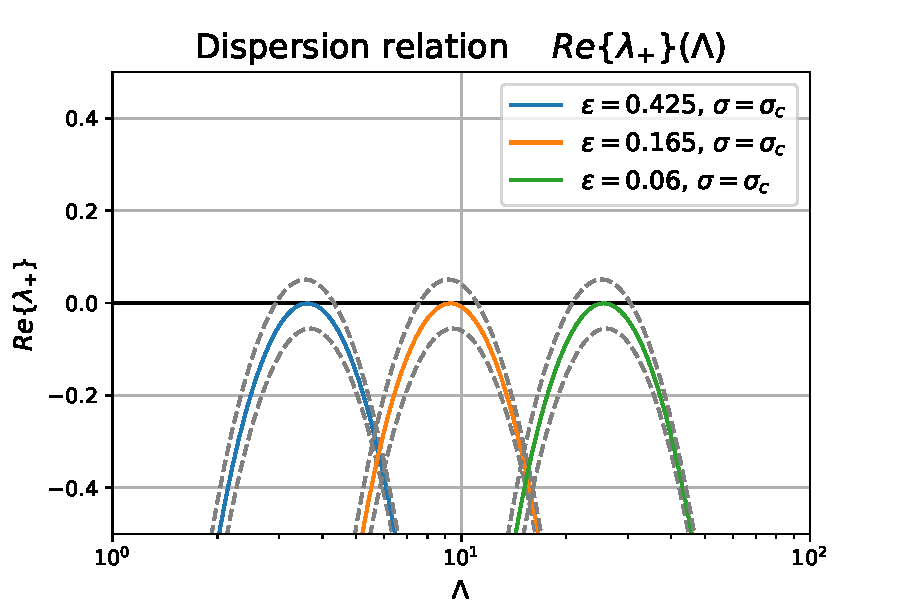
\includegraphics[width=0.8\textwidth]{latex_source/images/simulations/multiple_dispersion.pdf}
    \caption{Dispersion relation for the chosen reaction kinetics [Eq. $\ref{eq:chosen_kinetics}$], at different values of the activator diffusivity $\epsilon$. The dashed grey lines are the dispersion curves slightly above and below the critical diffusivity ratio $\sigma_c$. As stated in [Eq. \ref{eq:critical_eigenvalue}], the critical eigenvalue $\Lambda_c$ is inversely proportional to the activator diffusivity $\epsilon$.}
\end{figure}
Following the choice of the authors, I simulated the dynamics on Barabasi-Albert scale free networks. I chose parameters $N = 200$ for the number of nodes and $\<k\> = 10$ for the mean degree. My activator diffusivity was $\epsilon = 0.12$, and my diffusivity ratio was $\sigma = 15.6 > \sigma_c = 15.5$. The reasoning for chosing a diffusivity ratio that is only slightly above the critical threshold is to keep the number of different allowed modes low.
\begin{figure}[H]
\subfigure[]{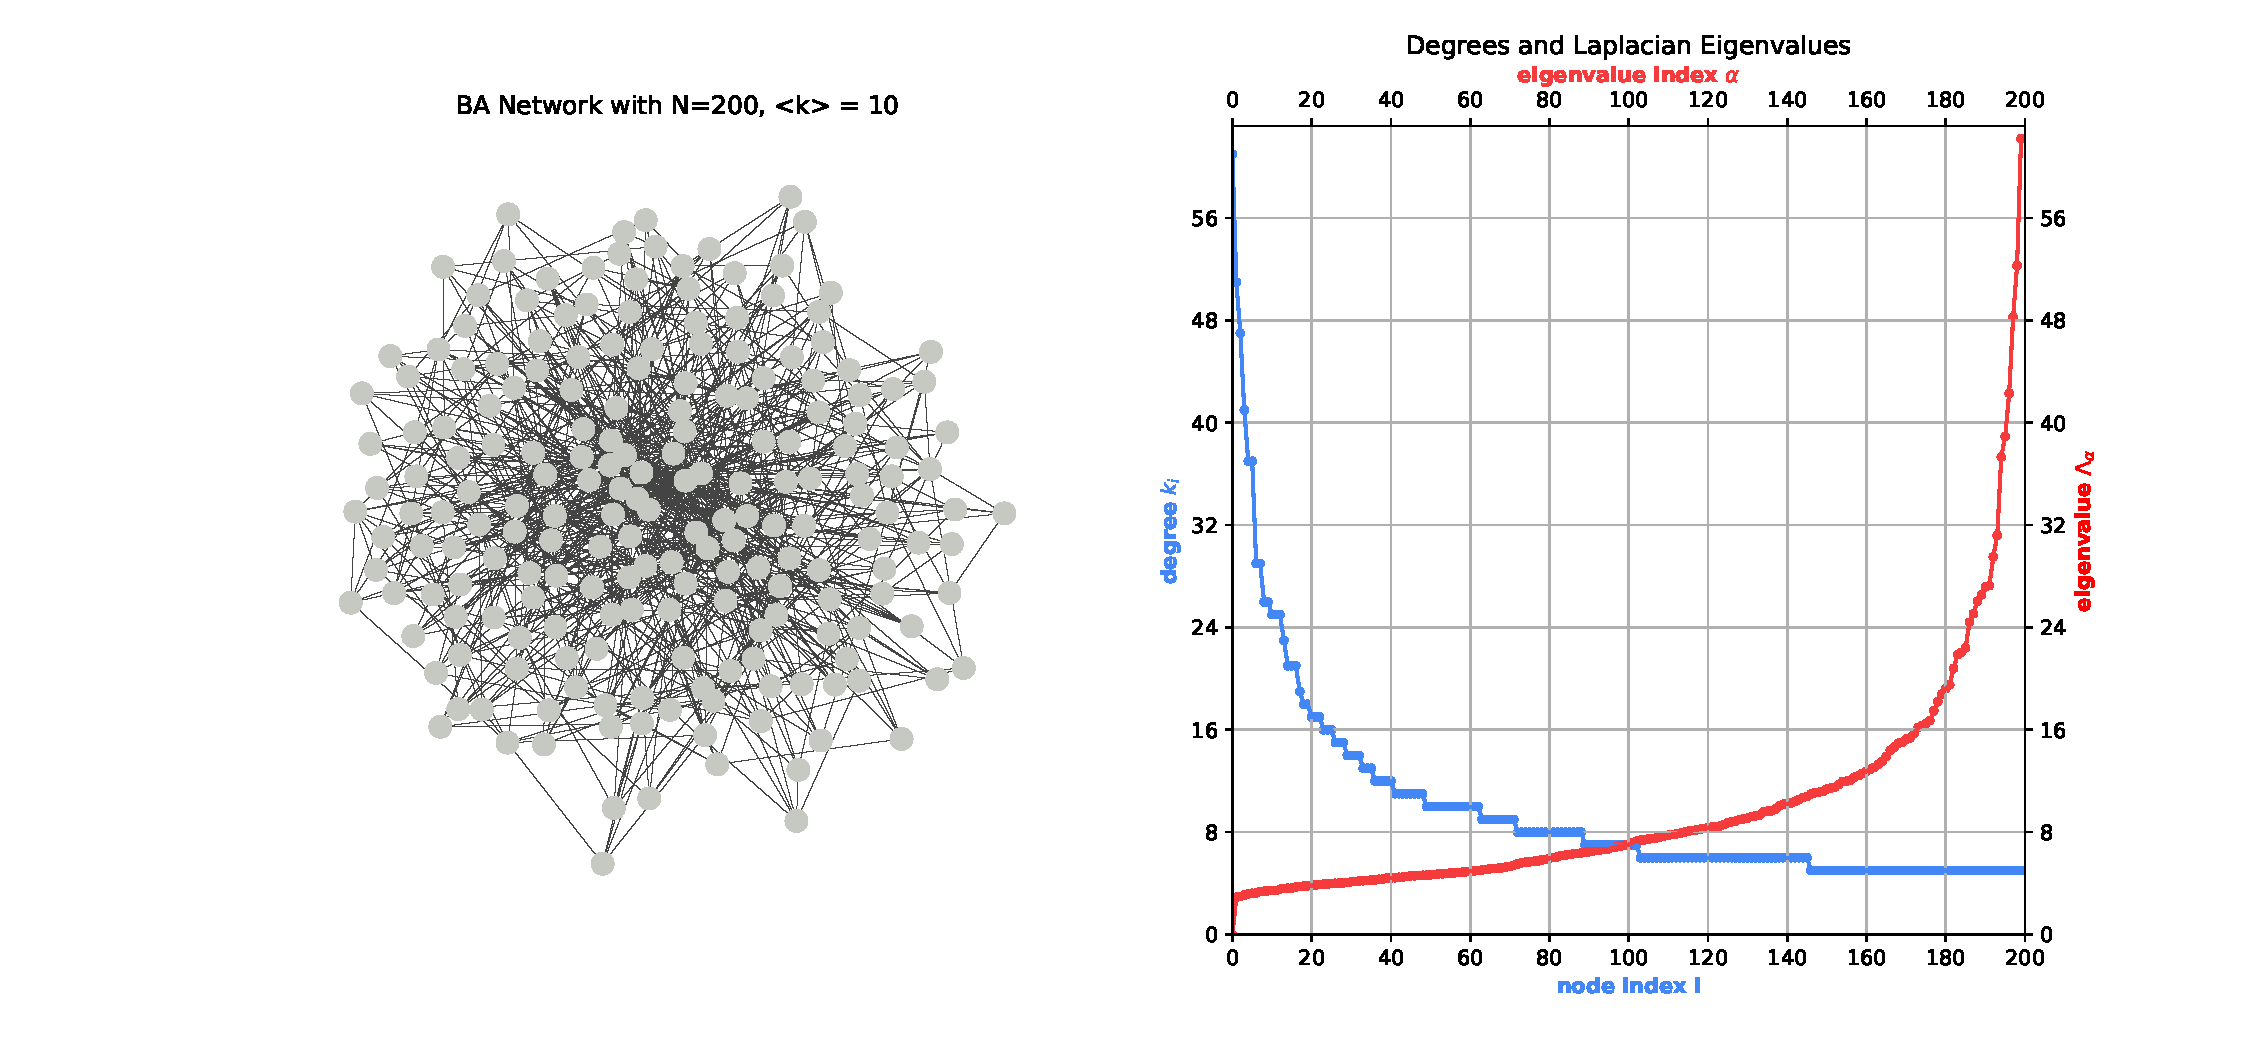
\includegraphics[width = 0.47\textwidth]{latex_source/images/simulations/network_200.pdf}}
\subfigure[]{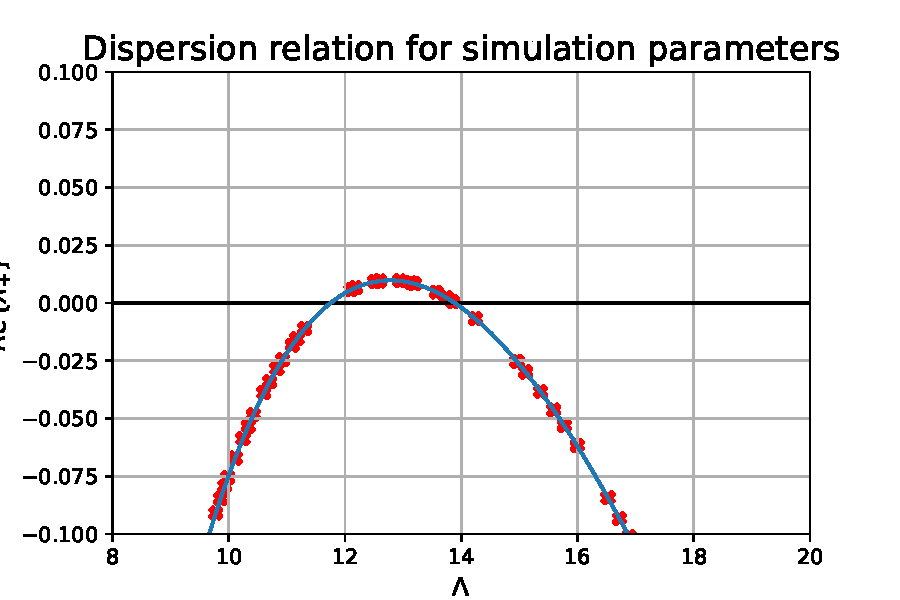
\includegraphics[width = 0.47\textwidth]{latex_source/images/simulations/simulation_dispersion.pdf}}
\caption{Most relevant properties of the network used in the simulation. Subfigure (a) shows the degree spectrum and the laplacian eigenvalue spectrum of the chosen graph. Network nodes are indexed by decreasing degree. Subfigure (b) shows the dispersion relation curve. Critical eigenvalue is $\Lambda_c \simeq 12.8141$. The eigenvalue closest to $\Lambda_c$ is $\Lambda_n \simeq 12.64$, of index $n=157$. However, as one can see from the graph, the network eigenvalue spectrum comprehends several other allowed modes (red crosses) in the unstable range, and they are expected to contribute to pattern initiation as well.}
\end{figure}
\noindent
The initial homogeneous state $(\overline{u},\,\overline{v})$ was perturbed with a random uniform perturbation at each node of amplitude $0.05$. [Figure \ref{fig:snapshots}] show snapshots of the activator concentration on nodes at different times. Also, the GithHub repository \cite{git} contains a .mp4 video of the whole evolution. \medskip \newline \noindent
In the early stage, the pattern is expected to grow proportionally to the critical eigenvector, which is is the mode of largest growing rate: $\delta\,u(t),\, \delta\,v(t) \propto \Phi^{(n)}$.
In fact, when the initial uniform perturbation dies out and the pattern starts to grow, the activator substance distribution is located similarly to the critical eigenvector (see snapshot $t = 25.06$). Later on, the evolution becomes strongly non-linear and the pattern is reshaped (see snapshot at $t = 100.25$), till it settles into a stationary state (see snapshot at $t = 150.38$) where nodes are split into one activator-rich group and one activator-poor group. The authors found that this peculiar behaviour is well described in the framework of a mean field theory \cite{main_network}. \medskip \newline \noindent
An interesting thing one can notice in the initial stage pattern [Figure \ref{fig:snapshots}, snapshot at $t = 25.06$] is that the significant variations of the activator level are localized on a subset of nodes of close degree ($k \sim 25-75$). That is, only a specific subset of the network undergoes differentiation. This effect is was not a fortuity but is due to the fact that the laplacian eigenvectors in a large graph with a broad degree distribution tend to be localized around a specific degree $\overline{k}(\Lambda)$. Also, as authors report, a simple relation $\overline{k}(\Lambda) \simeq \Lambda$ seems to hold. I checked wether I could find the same behaviour for my graph (see [Figure \ref{fig:eigenvectors}] and [Figure \ref{fig:heatmap}].
\begin{figure}[H]
    \centering
    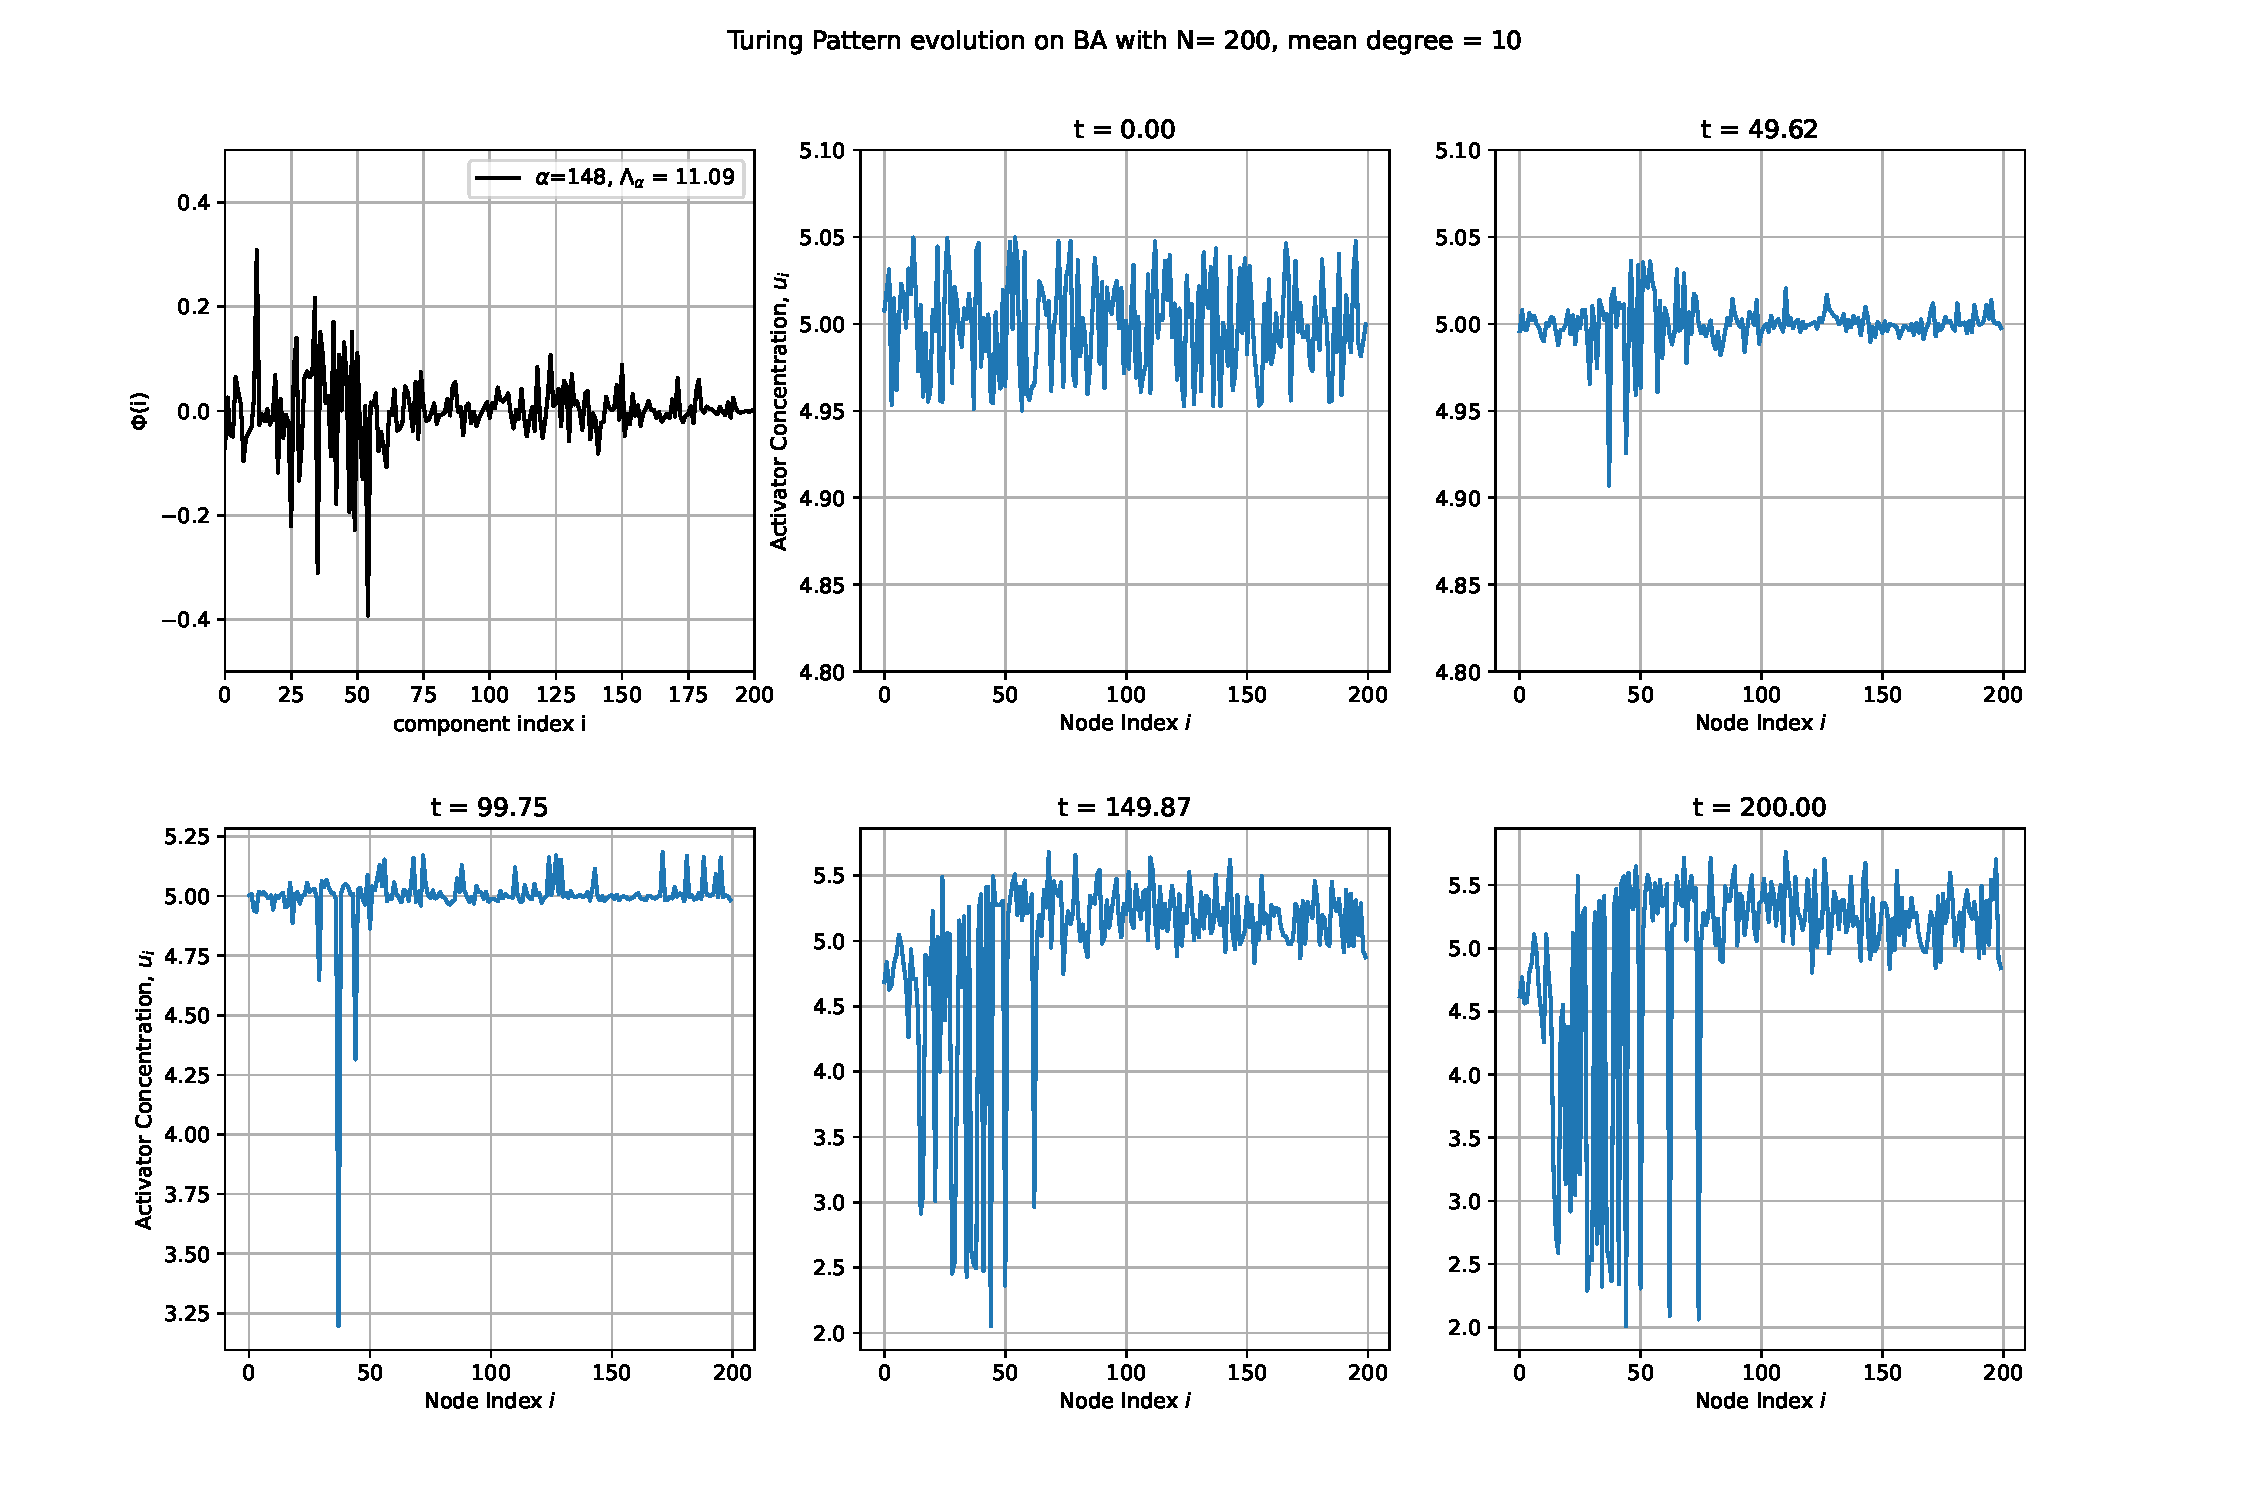
\includegraphics[width = 0.9\textwidth]{latex_source/images/simulations/snapshots.pdf}
    \caption{Time evolution of the activator concentration. The subfigure at top left corner shows the components of the critical eigenvector (in black) and its closest neighbours in the unstable range (in grey).}
    \label{fig:snapshots}
\end{figure}
\begin{figure}[H]
\centering
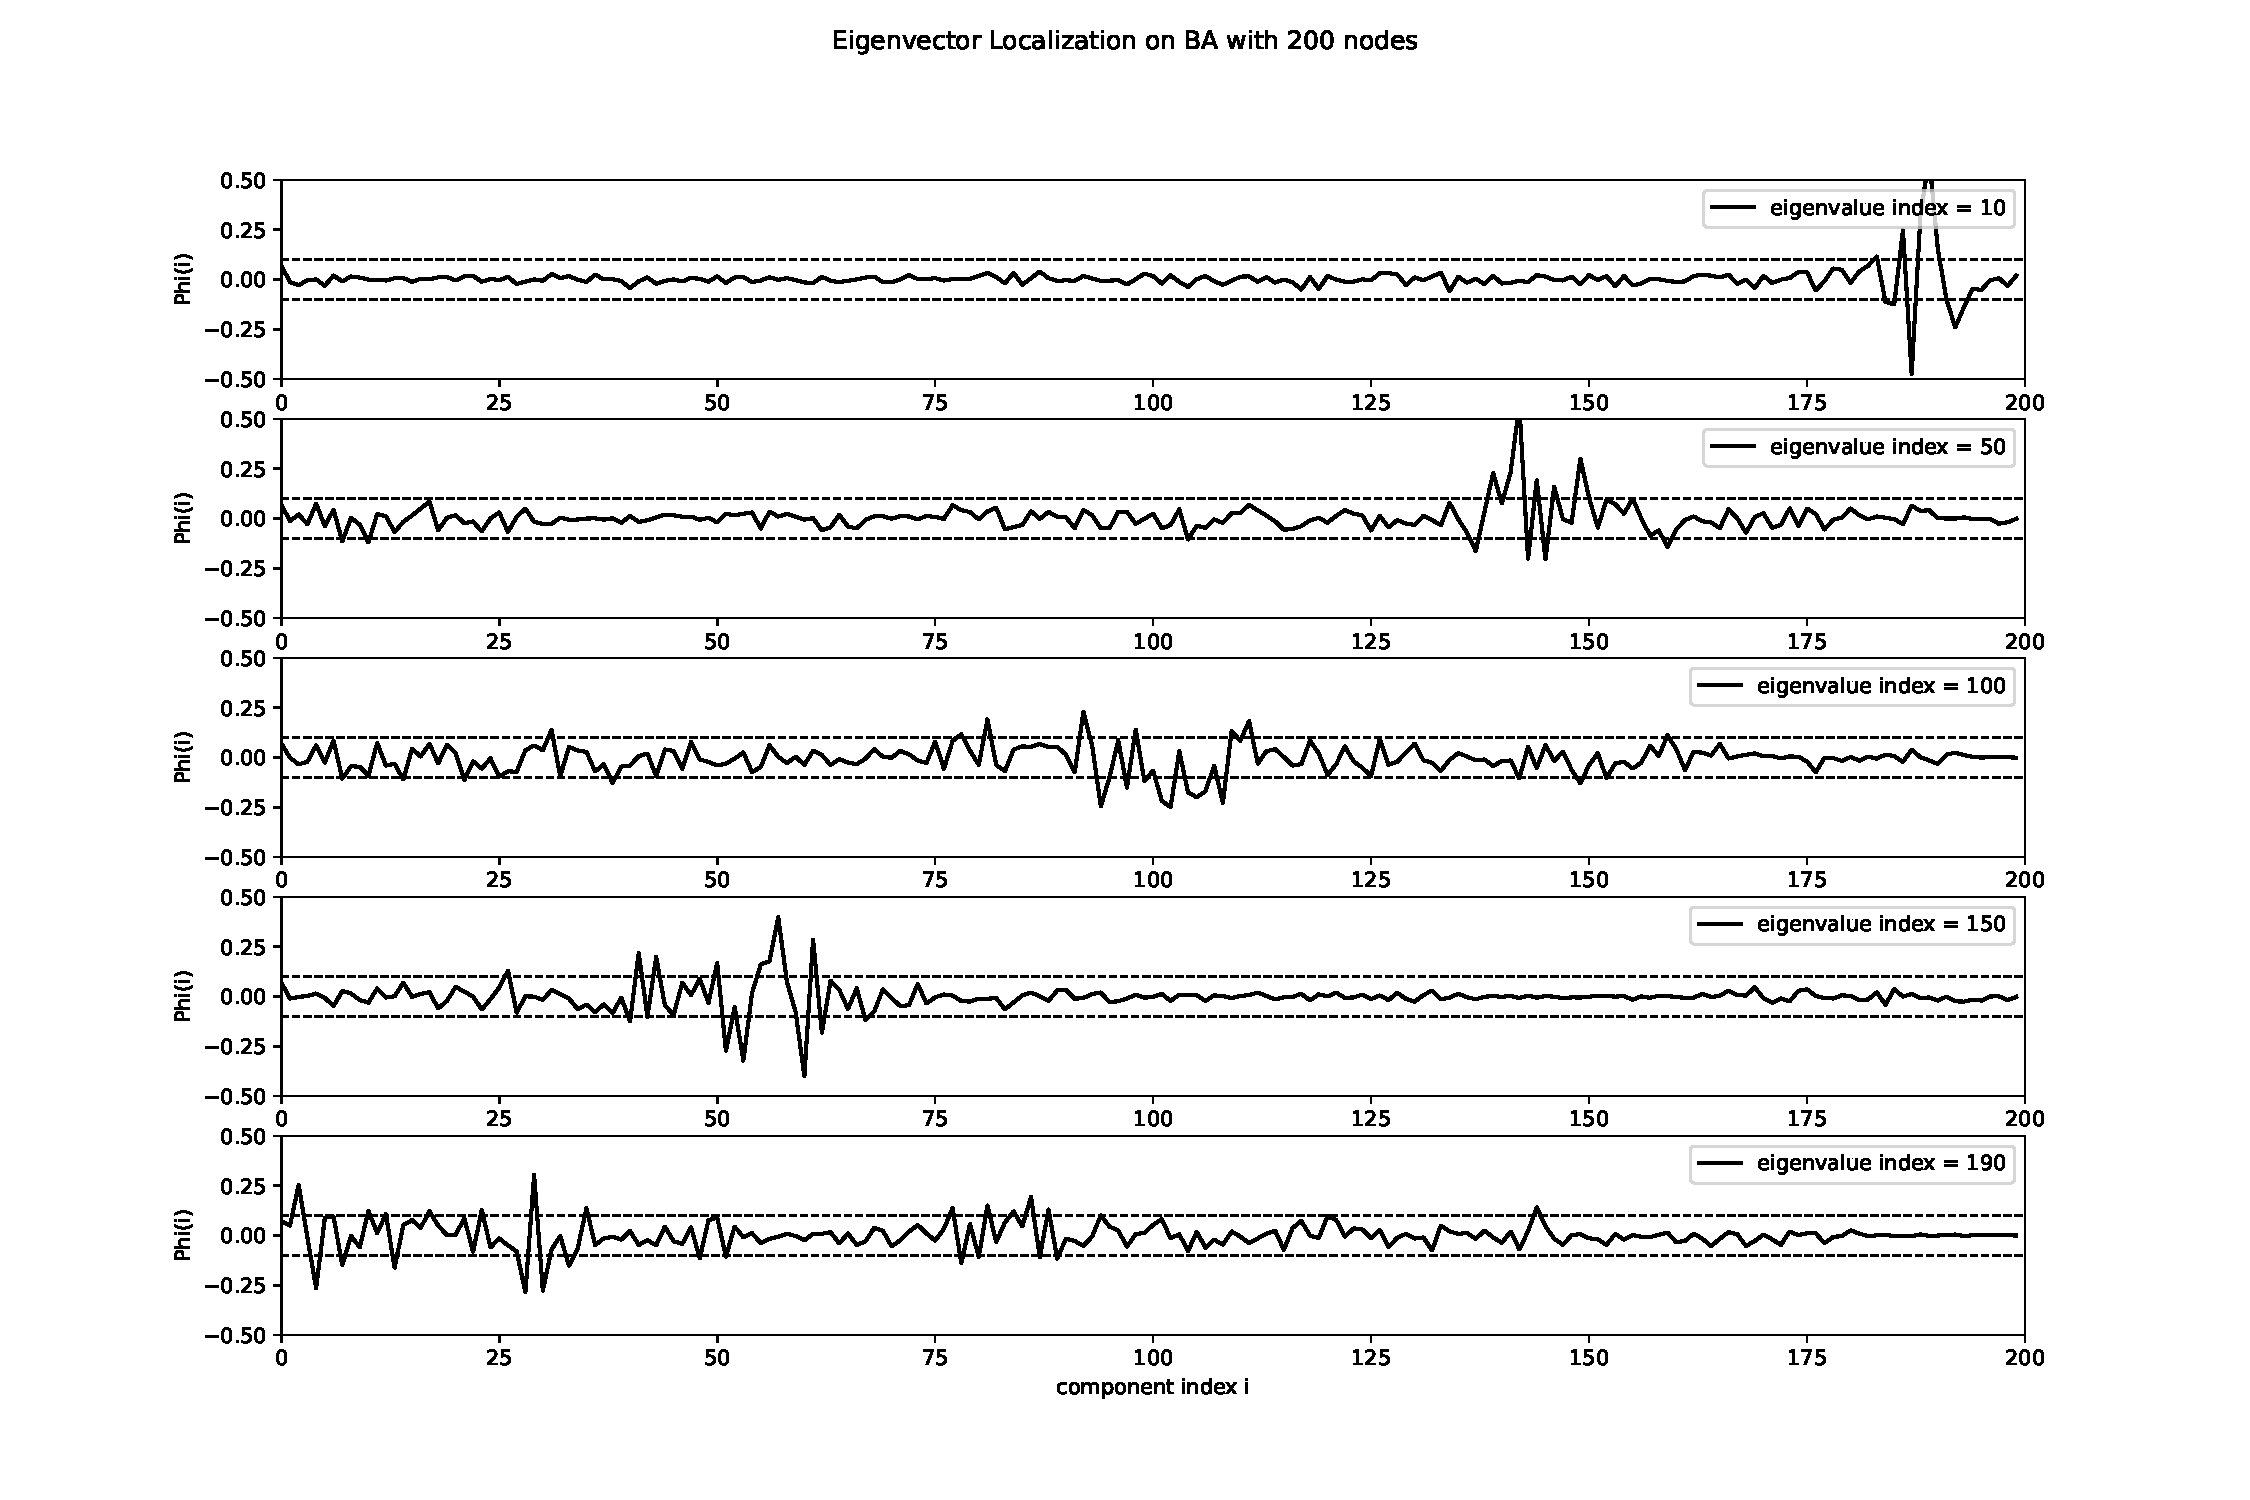
\includegraphics[width =\textwidth]{latex_source/images/simulations/eigenvectors_200.pdf}
\caption{Localization of laplacian eigenvectors in 
a BA with $N=200$ and $\<k\> = 10$. Nodes nodes are ranked by their degree. With incrementing eigenvalue $\Lambda$, the characteristic degree becomes higher.}
\label{fig:eigenvectors}
\end{figure}

\begin{figure}[H]
    \centering
\subfigure[]{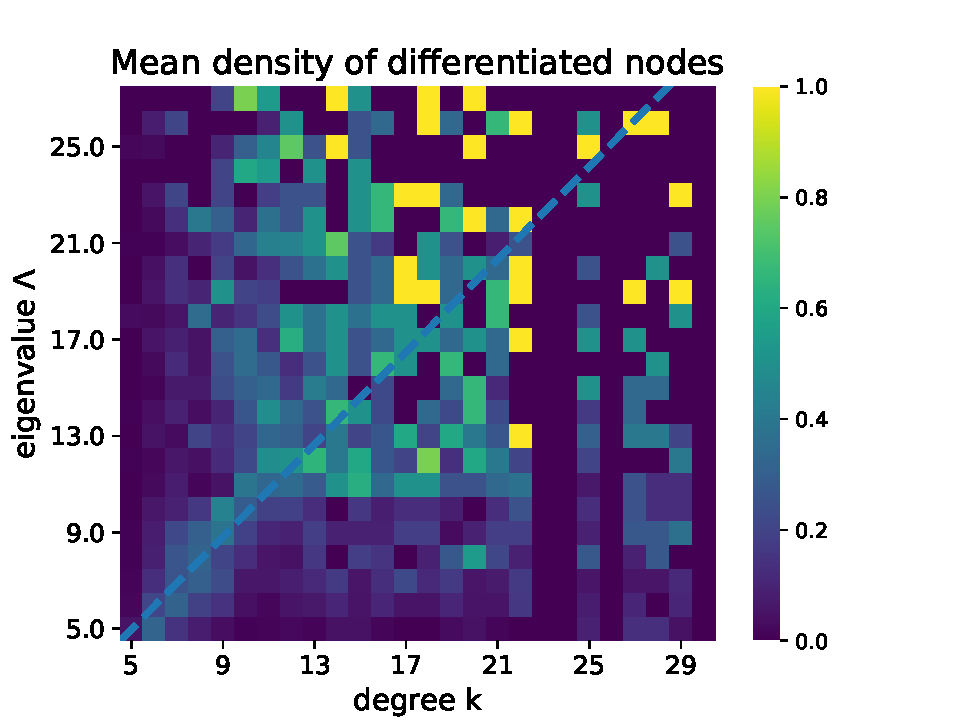
\includegraphics[width=0.48\textwidth]{latex_source/images/simulations/density_200.pdf}}
\subfigure[]{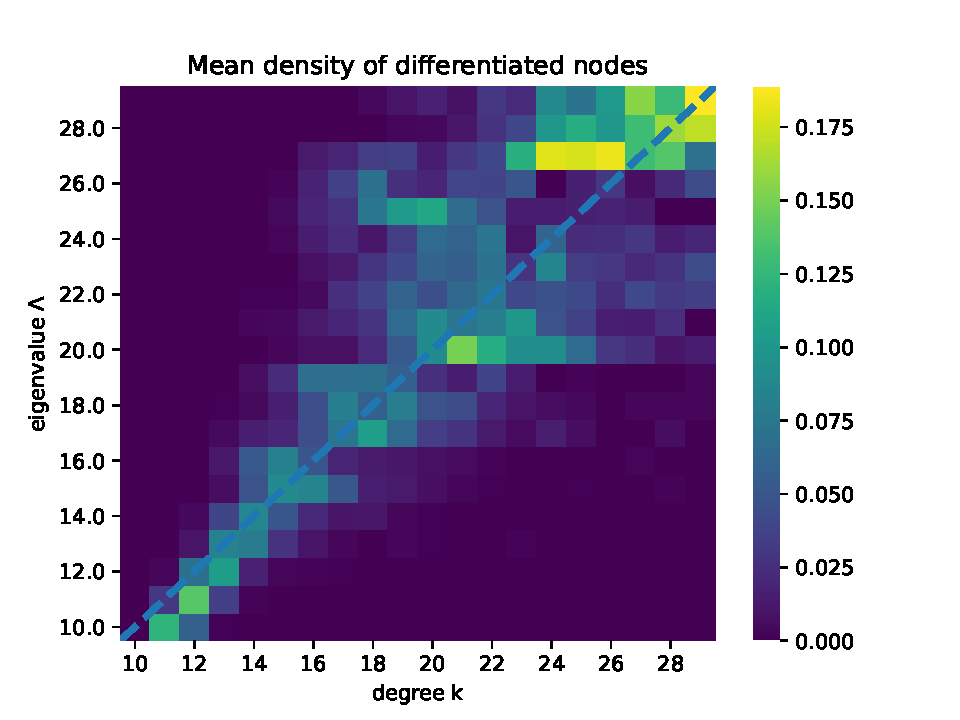
\includegraphics[width=0.48\textwidth]{latex_source/images/simulations/density_1000.pdf}}
\caption{Localization of laplacian eigenvectors in a BA graph with $N=200$ nodes and $\<k\>=10$ (a) and in a BA graph with $N=1000$ nodes and $\<k\>=20$ (b). Eigenvalues have been grouped into bins of unitary width. The population of nodes inside each degree group, $N_k$, was calculated. The heatmap represents the mean density of differentiated nodes for each degree group $z = N_k^{\text{diff}}(\Lambda)/N_k$. A node $i$ of degree was considered to be differentiated with respect to eigenvalue $\Lambda_n$ if its eigenvector component satisfied, $|\Phi_i^{(n)}|> 0.1$. I found, like authors \cite{main_network} report, that approximately $\overline{k}(\Lambda) \propto \Lambda$ (dashed line) and that effect is more pronounced in the larger graph.}
\label{fig:heatmap}
\end{figure}
